%% 
%% Copyright 2007-2024 Elsevier Ltd
%% 
%% This file is part of the 'Elsarticle Bundle'.
%% ---------------------------------------------
%% 
%% It may be distributed under the conditions of the LaTeX Project Public
%% License, either version 1.3 of this license or (at your option) any
%% later version.  The latest version of this license is in
%%    http://www.latex-project.org/lppl.txt
%% and version 1.3 or later is part of all distributions of LaTeX
%% version 1999/12/01 or later.
%% 
%% The list of all files belonging to the 'Elsarticle Bundle' is
%% given in the file `manifest.txt'.
%% 
%% Template article for Elsevier's document class `elsarticle'
%% with numbered style bibliographic references
%% SP 2008/03/01
%% $Id: elsarticle-template-num.tex 249 2024-04-06 10:51:24Z rishi $
%%
\documentclass[preprint,12pt]{elsarticle}

%% Use the option review to obtain double line spacing
%% \documentclass[authoryear,preprint,review,12pt]{elsarticle}

%% Use the options 1p,twocolumn; 3p; 3p,twocolumn; 5p; or 5p,twocolumn
%% for a journal layout:
%% \documentclass[final,1p,times]{elsarticle}
%% \documentclass[final,1p,times,twocolumn]{elsarticle}
%% \documentclass[final,3p,times]{elsarticle}
%% \documentclass[final,3p,times,twocolumn]{elsarticle}
%% \documentclass[final,5p,times]{elsarticle}
%% \documentclass[final,5p,times,twocolumn]{elsarticle}

%% For including figures, graphicx.sty has been loaded in
%% elsarticle.cls. If you prefer to use the old commands
%% please give \usepackage{epsfig}

%% The amssymb package provides various useful mathematical symbols
\usepackage{amssymb}
%% The amsmath package provides various useful equation environments.
\usepackage{amsmath}
\usepackage{booktabs}
\usepackage{hyperref}

\usepackage[percent]{overpic}
%% The amsthm package provides extended theorem environments
%% \usepackage{amsthm}

%% The lineno packages adds line numbers. Start line numbering with
%% \begin{linenumbers}, end it with \end{linenumbers}. Or switch it on
%% for the whole article with \linenumbers.
%% \usepackage{lineno}

\journal{Computers \& Fluids}

\begin{document}

\begin{frontmatter}

%% Title, authors and addresses

%% use the tnoteref command within \title for footnotes;
%% use the tnotetext command for theassociated footnote;
%% use the fnref command within \author or \affiliation for footnotes;
%% use the fntext command for theassociated footnote;
%% use the corref command within \author for corresponding author footnotes;
%% use the cortext command for theassociated footnote;
%% use the ead command for the email address,
%% and the form \ead[url] for the home page:
%% \title{Title\tnoteref{label1}}
%% \tnotetext[label1]{}
%% \author{Name\corref{cor1}\fnref{label2}}
%% \ead{email address}
%% \ead[url]{home page}
%% \fntext[label2]{}
%% \cortext[cor1]{}
%% \affiliation{organization={},
%%             addressline={},
%%             city={},
%%             postcode={},
%%             state={},
%%             country={}}
%% \fntext[label3]{}

\title{Limits of POD-based Sparse Pressure Reconstruction in Wall-confined Cylinder Wakes: Gap-regime Unsteady Reconstruction Assessment}

%% use optional labels to link authors explicitly to addresses:
%% \author[label1,label2]{}
%% \affiliation[label1]{organization={},
%%             addressline={},
%%             city={},
%%             postcode={},
%%             state={},
%%             country={}}
%%
%% \affiliation[label2]{organization={},
%%             addressline={},
%%             city={},
%%             postcode={},
%%             state={},
%%             country={}}

\author[aff1]{Bastien Lagneaux}
\author[aff1]{Corentin Porcon}
\author[aff1]{Florence Razan}
\author[aff2]{Dixia Fan}
\author[aff1]{Gurvan Jodin\corref{cor1}}
\cortext[cor1]{Corresponding author email address: gurvan.jodin@ens-rennes.fr}

%% Author affiliation
\affiliation[aff1]{organization={Univ Rennes, ENS RENNES, CNRS IETR - UMR 6164},%Department and Organization
            city={Rennes},
            country={France}}

\affiliation[aff2]{organization={Engineering Department, Westlake University},%Department and Organization
            addressline={Zhejiang}, 
            country={China}}

%% Abstract
\begin{abstract}
Proper orthogonal decomposition (POD) is often used as an interpretable front-end for sparse flow reconstruction and data fusion, but its reliability is uncertain when the wake is wall-confined, transient and regime-dependent. This study tests that reliability on a controlled two-dimensional computational data set of a circular cylinder in a finite rectangular tank. Reynolds number, wall proximity, spatial windowing, grid resolution and body translation are varied to diagnose full-field POD reconstruction error. A second benchmark then evaluates pressure reconstruction from eight synthetic wall-mounted pressure sensors using mean-field reconstruction, global and regime-local full-field POD projection, global gappy POD and regime-local gappy POD. The full-field results show that, over the sampled range $Re=10^3-10^4$, reconstruction error is much more sensitive to wall proximity than to Reynolds number. The most confined wakes also lose the quasi-periodicity exploited in canonical cylinder-wake POD analyses. In the pressure benchmark, global full-field POD reduces the average pressure normalized Frobenius error from 1.04 for the mean field to 0.13, while regime-local full-field POD gives a comparable value of 0.12. Global wall-sensor gappy POD reaches 0.86, and regime-local gappy POD improves this value to 0.73, although its worst errors remain concentrated near regime boundaries. These results show that energy retention, local bases and wall-sensor fit are not sufficient by themselves to guarantee robust sparse observability in confined wakes.
\end{abstract}

%%Graphical abstract
%\begin{graphicalabstract}
%\includegraphics{grabs}
%\end{graphicalabstract}

%%Research highlights
%\begin{highlights}
%\item A 2D confined-cylinder benchmark probes POD limits for sparse fusion.
%\item Wall gap dominates POD reconstruction error across sampled cases.
%\item Eight wall-pressure sensors give limited full-field observability.
%\item Regime-local POD improves pressure reconstruction.
%\item Energy retention and sensor fit are weak robustness indicators.
%\end{highlights}

%% Keywords
\begin{keyword} 
proper orthogonal decomposition; gappy POD; sparse sensing; data fusion; wall-bounded wake; cylinder flow
%% keywords here, in the form: keyword \sep keyword

%% PACS codes here, in the form: \PACS code \sep code

%% MSC codes here, in the form: \MSC code \sep code
%% or \MSC[2008] code \sep code (2000 is the default)

\end{keyword}

\end{frontmatter}

%% Add \usepackage{lineno} before \begin{document} and uncomment 
%% following line to enable line numbers
%% \linenumbers

%% main text
%%

%% Use \section commands to start a section
\section{Introduction}
\label{sec1}
%% Labels are used to cross-reference an item using \ref command.

Sparse reconstruction of unsteady flow fields is a central challenge in fluid mechanics when only limited experimental measurements are available. In many applications, time-resolved sensor signals can be acquired more easily than spatially resolved velocity or pressure fields, while numerical simulations can provide complete fields at the cost of modeling assumptions and computational expense. Reduced-order modeling (ROM) offers a natural framework for connecting these two sources of information: sparse measurements can be used to describe the low-dimensional state of the flow, and this state can then be mapped back to a full-field estimate.

A closely related sensor-based sparse-ROM perspective was developed by Loiseau et al.~\citep{Loiseau2017}, who proposed a sparse reduced-order modeling framework in which time-resolved sensor data are lifted to a low-dimensional feature space, sparse nonlinear dynamics are identified in that space using SINDy, and, when full-state snapshots are available, the feature state is mapped to the full flow field. This strategy is attractive for experimental fluid mechanics because it does not require time-resolved full-field measurements and because the identified dynamics can remain interpretable. It also highlights a key requirement for sparse flow reconstruction: the mapping between sensor information, reduced coordinates and full-state fields must remain stable when the flow geometry, boundary conditions or operating regime changes.

Proper orthogonal decomposition (POD) remains one of the most common tools for constructing such reduced representation. POD provides an energy-optimal basis for a given snapshot ensemble and yields interpretable coherent structures \citep{Berkooz1993,Chatterjee2000}. It is particularly successful in canonical cylinder wakes with well-established periodic vortex shedding \citep{Noack2003,Tadmor2010}. Recent work in non-intrusive model reduction for vortex-induced vibrations further illustrates that POD remains a relevant building block for wake ROMs, while also emphasizing robustness with respect to model dimension and operating conditions \citep{Gkimisis2024}. POD is therefore a natural baseline candidate for the modal full-state reconstruction stage of sparse reduced-order modeling, and gappy POD provides a direct way to estimate modal coefficients from incomplete measurements \citep{Willcox2006}.

However, the reliability of this strategy is uncertain when the flow is confined, transient and regime-dependent. POD bases are constructed from the data on which they are trained, and their validity can degrade when the spatial structure of the flow changes. This limitation is especially relevant near solid boundaries. For a circular cylinder close to a wall, wall proximity modifies the wake topology, suppresses or distorts vortex shedding, and introduces proximity-dependent regimes that are absent in unbounded configurations \citep{Price2002,Chakraborty2004,Rao2013}. Under such conditions, high retained POD energy does not necessarily imply that the resulting modes provide a robust basis for sparse reconstruction or for downstream dynamical modeling.

The present study is motivated by hydrodynamic sensing in confined experimental tanks. In biological flow-sensing applications, wall-mounted pressure sensors can provide sparse but physically grounded measurements, while simplified computational models can provide complete pressure, velocity and vorticity fields. The HAACHAMA pipeline, for example, combines video-based body kinematics, wall-pressure measurements and two-dimensional CFD simulations in a tank-like geometry \citep{Porcon2024,Lagneaux2025}. In such settings, freely swimming fish may accelerate, stop, turn or move close to the tank wall, so both flow speed and wall proximity can vary during a trial. In order to enable behavioral study of how fish use the hydrodynamic cues left behind a previous specimen, full-field hydrodynamic maps fusing sensors sprase high-fidelity to simulation low-fieldity full-field estimation are needed. The biological application provides the motivation, while the computational issue addressed here is broader: sparse wall measurements must be related to full pressure and flow fields when the wake is wall-bounded, transient, and regime-dependent.

This paper tests a prerequisite for sensor-based sparse reduced-order modeling: the robustness and observability of POD-based full-field representations in a confined wake. More advanced modal decompositions and sensing strategies could also be considered. Frequency-aware decompositions such as SPOD \citep{Sieber2016,Towne2018} and mPOD \citep{Mendez2019,Mendez2020}, sparse extensions such as gappy SPOD \citep{Nekkanti2022}, and optimized sensor-placement methods \citep{Manohar2018,Sashittal2021} are natural candidates for improving reconstruction in wall-confined wakes. These methods are not excluded because they are irrelevant. Rather, they answer a different and more specialized question. The present study focuses on classical POD and gappy POD because they remain widely used, interpretable, and straightforward to deploy as first-line reduced-order tools in experimental data-fusion workflows. The objective is therefore to test whether this common baseline is already reliable enough to support sparse wall-pressure reconstruction before moving to more specialized alternatives, addressing a gap in the available literature: to the authors' knowledge, classical POD/gappy POD has not been systematically assessed for the combined setting of transient wall-confined wakes, varying wall proximity, regime-dependent flow structure, and full-field reconstruction from wall-mounted pressure samples, as encountered in organic swimming trajectories.

The contribution is twofold. First, the study provides an in-sample POD sensitivity diagnostic showing how Reynolds number, wall proximity, spatial windowing, grid resolution and body translation affect POD reconstruction error. Second, it provides a held-out sparse wall-pressure reconstruction benchmark comparing mean-field reconstruction, global and regime-local full-field POD projection, global gappy POD and regime-local gappy POD from eight wall sensors. Together, these analyses define the conditions under which classical POD and gappy POD provide, or fail to provide, a stable baseline for sparse sensor-to-full-state estimation in confined wakes.

\section{Background}
\label{sec2}
%% Use \subsection commands to start a subsection.
\subsection{Data-fusion context}
\label{subsec2.1}

The motivating HAACHAMA workflow uses two information sources. The first consists of sparse but high-fidelity pressure measurements acquired from sensors mounted along the tank wall \citep{Porcon2024}. The second is a low-fidelity digital twin generated with the LilyPad platform \citep{Maertens2015}, which produces pressure, velocity and vorticity fields on a two-dimensional grid. 

The intended fusion task is to retain the spatial completeness of the simulated fields while correcting them with physically measured pressure information. In this setting, wall-pressure sensors provide experimentally grounded observations, whereas the numerical model supplies full-field structure that cannot be measured directly at comparable spatio-temporal resolution. The resulting problem is therefore a sparse state-estimation problem in a confined wake, where incomplete wall measurements must be related to full pressure and flow fields despite modeling error, wall effects and changing flow regimes.

\subsection{Proper orthogonal decomposition}
\label{subsec2.2}
POD constructs a low-dimensional linear representation of a flow field by decomposing a set of snapshots into orthogonal spatial modes ordered by decreasing energy content. Given a flow field $u(x,t)$ and a truncation $r$, POD approximates its evolution as $u(x,t) \approx \sum\nolimits_{i=1}^r a_i(t)\,\phi_i(x)$ where $\phi_i(x)$ are the spatial modes, and $a_i(t)$ are modal coefficients. When applied to canonical flows such as unbounded cylinder wakes, this decomposition yields compact representations dominated by a small number of coherent structures \citep{Noack2003,Tadmor2010}.

Though complex problems such as water-entry of a cylinder have been successfully modeled using POD \citep{Sha2023}, the effectiveness of this representation relies on assumptions of dynamical coherence and regime consistency \citep{Loiseau2021}, which may be violated under strong confinement or transient conditions.

\subsection{SINDy and ROM interpretability}
\label{subsec2.3}
The sparse identification of nonlinear dynamics (SINDy) framework identifies compact dynamical systems from time series by sparse regression on a candidate library \citep{Brunton2016}. Applied to POD coefficients, SINDy requires a stable and sufficiently smooth reduced state. Variations in POD bases caused by wall effects, transients or changes of operating condition directly compromise the interpretability and predictive value of the identified equations. The SINDy discussion is therefore retained only as downstream motivation: the present paper tests whether the reduced coordinates supplied to such methods are stable enough to justify later inference.

\subsection{Wall-induced regimes and reduced representations}
\label{subsec2.4}
Studies of a circular cylinder near a wall have identified gap-dependent regimes characterized by changes in vortex shedding, force coefficients and wake topology \citep{Price2002,Chakraborty2004,Rao2013}. Price et al.~\citep{Price2002} separated the fixed-wall wake into very-small-gap, small-gap, intermediate-gap and large-gap regions: at the smallest gaps the gap flow is suppressed and regular vortex shedding is lost, at intermediate gaps vortex shedding begins to reappear, and at larger gaps the flow around the cylinder is basically unchanged by the wall. Later PIV measurements showed that decreasing gap ratio makes the wake increasingly asymmetric, promotes secondary vortices near the wall and produces irregular shedding below a critical gap \citep{He2017}. These works clarify the physics of wall-confined wakes, but they do not directly answer whether regime transitions translate into smooth variations in a POD basis or into representation instabilities. The present work addresses this representational question and then tests whether wall-pressure observations can recover the associated full pressure fields through gappy POD.

\section{Methods}
\label{sec3}
\subsection{Synthetic data set: cylinder in a finite rectangular tank}
\label{subsec3.1}
The final target system in this study, a fish, exhibits highly dynamic behavior, involving continuous shape deformation along smooth, organic trajectories. As a result, both swimming speed and proximity to the wall vary over time. However, for the purposes of the present investigation, a simplified CFD dataset was employed in which these complexities were excluded. The Reynolds number, representing speed (under the assumption that all other parameters are constant in $Re=U\cdot L/\nu$), and wall proximity were held fixed for each simulation. No body deformation was introduced, and the geometry was simplified to a rigid cylinder.

Numerically, the simulations were conducted in a two-dimensional tank with dimensions of 2 meters in length and 1 meter in width, with incoming flow imposed from the left boundary. These dimensions were chosen to facilitate reproducibility and to ensure compatibility with potential future experimental validation. The cylinder diameter was fixed at 0.05 meters, consistent with the characteristic scale of small aquatic animals such as striped eel catfish Plotosus lineatus, while maintaining a ratio of at least 10:1 between tank half-width and cylinder diameter. This configuration approximated an effectively unbounded far side while retaining a nearby wall for the confinement study.

The cylinder was positioned at two-sevenths of the tank length from the left boundary, allowing sufficient upstream distance for the establishment of a steady incoming flow while preserving most of the domain for the development of a von Karman vortex street. Each simulation was run for a duration of 500 time units, with time steps defined by the relation (all quantities being expressed in non-dimensional form using the grid size and the uniform flow velocity as reference scale):
\begin{align}
    \Delta t= \text{min}(\frac{1}{\text{max}_{i,j}(|u_x(i,j)|+|u_y(i,j)|) + 3\cdot\nu},1)
\end{align}
with $u_x(i,j)$ the horizontal velocity at grid point (i, j), $u_y(i,j)$ the vertical velocity at grid point (i, j) and $\nu$ the kinematic viscosity. 

The Reynolds number was varied across a range from $10^3$ to $10^4$, with simulation scenarios uniformly distributed within this interval. This range corresponds to realistic swimming speeds for fish while remaining feasible for replication in towing tank experiments. Similarly, the wall proximity, defined as the distance between the cylinder surface and the nearest tank wall $h$ and normalized by the cylinder diameter $D$, was varied from $h/D = 0.44$ to $h/D = 4.19$.

To investigate the impact of computational parameters (\hyperref[fig7]{figure~1}), the simulation window was progressively reduced in size by factors of 2 and 4 in both horizontal and vertical directions, effectively zooming in on the cylinder. This windowing strategy allowed for the evaluation of how restricting the field of interest to the immediate vicinity of the swimmer, while excluding distant boundaries or obstacles, affects POD performance. Narrowing the window is also relevant for realistic cases where a fish swims along organic trajectories: a sliding window centered on the animal changes the reference frame and moves the analysis closer to a local wake problem. Windowing was applied either a priori, by computing POD only on the reduced domain, or a posteriori, by applying POD to the full simulation and reconstructing the windowed region.

Additionally, the resolution of the CFD simulations was doubled for a subset of the dataset to examine the sensitivity of POD behavior to spatial discretization.

To further approach realistic conditions, a portion of the dataset was modified to include translational motion. In these cases, the cylinder was not stationary but traversed a 1-meter straight path from right to left through initially still fluid. Reynolds number and wall proximity were maintained as in the stationary cases, implying that simulation duration varied inversely with speed. To allow comparison with the default fixed-cylinder simulations, matched time-cropped versions of the stationary cases were also generated.

Reynolds number and wall proximity were varied independently throughout the dataset to isolate their respective effects on POD-based representations. Although circular-cylinder wakes undergo three-dimensional transitions at Reynolds numbers below the upper range considered here \citep{Williamson1996}, the present simulations are used as a controlled two-dimensional benchmark for representation robustness and sparse observability, not as a complete three-dimensional wake model. This approximation remains appropriate for the present hydrodynamic-sensing context: low-frequency disturbances generated by swimming fish have been shown to be well represented by coherent, nearly two-dimensional vortical structures \citep{Hanke2000}, and the Cartesian-grid method underlying LilyPad has been validated for Reynolds numbers up to $10^5$ \citep{Maertens2015}.

\begin{figure}[]
\centering{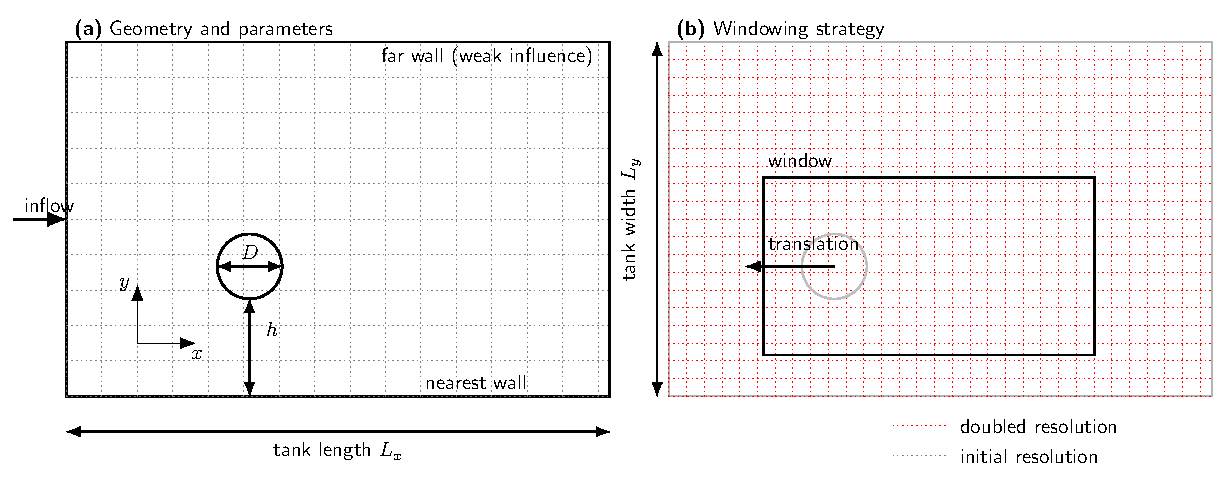
\includegraphics[width=0.75\linewidth]{figures/blueprint.pdf}}
\caption{Schematic of the computational configuration. (a) The cylinder of diameter D, at gap $h$ from the nearest wall, with imposed inflow direction. A coarse grid is the baseline spatial resolution. (b) Spatial window strategy. The finer grid is the doubled-resolution. The arrow indicates the direction of body translation in the moving-cylinder cases.}
\label{fig7}
\end{figure}

\subsection{In-sample POD sensitivity diagnostic}
\label{subsec3.2}
For each simulation time step, the pressure or vorticity fields were flattened into column vectors and assembled into a snapshot matrix. Prior to decomposition, the temporal mean was subtracted from each snapshot to ensure zero-centered data. POD was computed via singular value decomposition (SVD) \citep{Harris2020}. Since this POD analysis was an in-sample sensitivity diagnostic, for each configuration, the POD basis was computed from the full snapshot sequence and the same sequence was reconstructed. No train/test split was used in that stage, because the objective was to measure how the POD representation itself varies with Reynolds number, wall gap and numerical choices.


The number of retained modes corresponded to 99\% of the cumulative energy content. Reconstruction errors were quantified as the mean per snapshot root-mean-square error (RMSE) over the entire simulation duration.

To provide a reference for evaluation, results were compared against the canonical case of a fixed cylinder at Reynolds number $Re=10^2$ in an unbounded domain, as originally analyzed by Noack et al.~\citep{Noack2003}.

\subsection{Periodicity analysis}
\label{subsec3.4}
POD does not require periodic data in a strict mathematical sense, and has been applied to transient cylinder-wake measurements with frequency-varying vortex shedding, as in the study of Mendez et al.\citep{Mendez2020}. However, the more restrictive POD workflow used by Noack et al.\citep{Noack2003}, which is the reference for the present study, where the basis is built on an established periodic regime and supplemented by a shift mode, requires checking whether such a periodic regime exists in the present stationary-cylinder simulations. 

To assess the validity of this assumption under more realistic conditions, a periodicity analysis was performed on the most challenging case in the dataset defined as the scenario with the highest Reynolds number and the smallest wall proximity. Each simulation snapshot was flattened into a one-dimensional vector and correlated with the final snapshot of the simulation.

In a fully periodic system, peaks in correlation would be expected at intervals corresponding to vortex shedding cycles. Conversely, the absence of recurring peaks would indicate nonperiodicity and a breakdown of the cyclic behavior assumed in classical POD applications.

\subsection{Sensitivity tests performed}
\label{subsec3.5}
Four controlled test protocols were designed to assess the robustness of POD under varying physical and computational conditions.

In the first series of tests, the distance between the cylinder and the wall was held constant while the Reynolds number was incrementally varied to span the full range of values. This procedure was repeated for each discrete wall proximity value in the dataset.

The protocol was then reversed: the Reynolds number was fixed, and wall proximity was varied across its defined range.

These two stages of varying Reynolds number at fixed proximity, and varying proximity at fixed Reynolds number were subsequently applied in the three other tests corresponding to the previously mentioned subsections of the dataset: (i) simulations with spatial windowing, (ii) simulations with doubled spatial resolution, and (iii) translating-cylinder scenarios. 

\subsection{Held-out sparse wall-pressure reconstruction}
\label{subsec3.3}
Five pressure reconstructions were compared: the training mean field, global full-field POD projection, regime-local full-field POD projection, and global and regime-local wall-sensor gappy POD. The benchmark was performed on fixed-cylinder pressure snapshots from the same Reynolds number and wall-gap parameter space as the POD sensitivity analysis. Contiguous chronological split was avoided because the transient is localized at the beginning of simulations and assigning the first snapshots to training and the last snapshots to testing would therefore bias the evaluation toward late-time reconstruction. Roberts et al.~\citep{Roberts2017} emphasize that validation strategies for temporally structured data should be chosen according to dependence structure and prediction objective, often motivating blocked partitions. In the present benchmark, however, the temporal structure varies across Reynolds number, wall gap and flow regime, so a single block length would be arbitrary and would not guarantee comparable transient and late-time content across the 100 cases. 

A fixed-seed, case-wise randomized snapshot partition was therefore used. For each simulation, individual snapshots were assigned to training, validation and test sets with proportions 70\%, 15\% and 15\%, respectively, and the selected indices were then kept in chronological order within each subset. The same split was used for all reconstruction variants. After this case-wise partition, the training snapshots were concatenated across cases to build the POD bases. The global basis was fitted from the concatenated training snapshots of all 100 cases, whereas the regime-local bases were fitted from the concatenated training snapshots belonging to each gap-regime group. Training snapshots were used to compute the mean field and full-field POD ranks from the cumulative training variance, validation snapshots were used to select the gappy POD rank and ridge parameter, and final errors were computed on held-out test snapshots. This protocol estimates sparse reconstruction accuracy over the sampled trajectory rather than future-time forecasting performance.

The observation operator $H$ selected eight uniformly spaced pressure samples between $1/4^{th}$ and $3/4^{th}$ of the nearest wall to mimic the wall-mounted sensor configuration used in the experimental workflow.

The full-field projections are oracle diagnostics because they use the complete test pressure field to estimate modal coefficients. They measure basis representation quality before sparse observability is imposed. In wall-sensor gappy POD, only the sparse observations $y(t)=Hp(t)$ were available.

Following gappy POD formulation described by Brunton and Kutz~\citep{BruntonKutz2022}, the modal coefficients were estimated from the restriction of the pressure fluctuation to the measured wall-sensor support. Because only eight wall-pressure sensors were available, the least-squares problem was solved with optional ridge regularization,
\begin{align}
\hat{a}(t)=
\arg\min_a \left\|H\Phi_r a-\left(y(t)-H\overline{p}\right)\right\|_2^2
+\lambda \|a\|_2^2 ,
\end{align}
where $\Phi_r$ contains the first $r$ pressure POD modes, $\overline{p}$ is the training mean pressure field, $\hat{a}(t)$ is the estimated modal coefficient vector, and $\lambda$ is the ridge regularization parameter.

The regime-local methods used separate bases for the small, intermediate and large-gap groups identified from the POD sensitivity analysis, while retaining the same eight wall sensors for the gappy variant. For full-field POD, ranks were selected as the smallest number of modes accounting for 99\% of the training-set variance. For gappy POD, the retained rank was selected on the validation snapshots from one to eight modes, so that the number of estimated modal coefficients never exceeded the number of wall sensors. The ridge regularization strength was selected jointly with the gappy POD rank on the validation snapshots.

To compare reconstruction methods across cases with different fluctuation amplitudes, sparse reconstruction accuracy was measured on held-out test snapshots with the normalized Frobenius error
\begin{align}
\mathrm{nRMSE} =
\frac{\|P_{\mathrm{test}}-\widehat{P}_{\mathrm{test}}\|_F}
{\|P_{\mathrm{test}}-\langle P_{\mathrm{test}}\rangle_t\|_F}.
\end{align}
Here, $P_{\mathrm{test}}$ is the matrix of held-out pressure snapshots, with one pressure field per column, $\widehat{P}_{\mathrm{test}}$ is the corresponding reconstructed pressure matrix, and $\langle P_{\mathrm{test}}\rangle_t$ is the temporal mean of the held-out pressure snapshots. Values above one indicate errors larger than the intrinsic unsteady pressure fluctuations of the test case. The sensor residual and the condition number of $H\Phi_r$ were also recorded for the two gappy-POD variants to compare sensor-space fit and sparse observability.

\section{Results}
\subsection{Periodicity check for POD protocol}
Reference-frame correlation of the worst-case scenario, defined by the highest Reynolds number and smallest wall gap, did not reveal a clear sequence of recurring peaks approaching the final-state correlation level (\hyperref[fig1]{figure~2}). This result does not rule out oscillatory wake dynamics, but indicates that the full snapshot sequence did not provide a clean periodic segment comparable to the canonical cylinder-wake limit cycle. POD was therefore applied to the full snapshot sequence for all simulations.

\begin{figure}[]
\centering{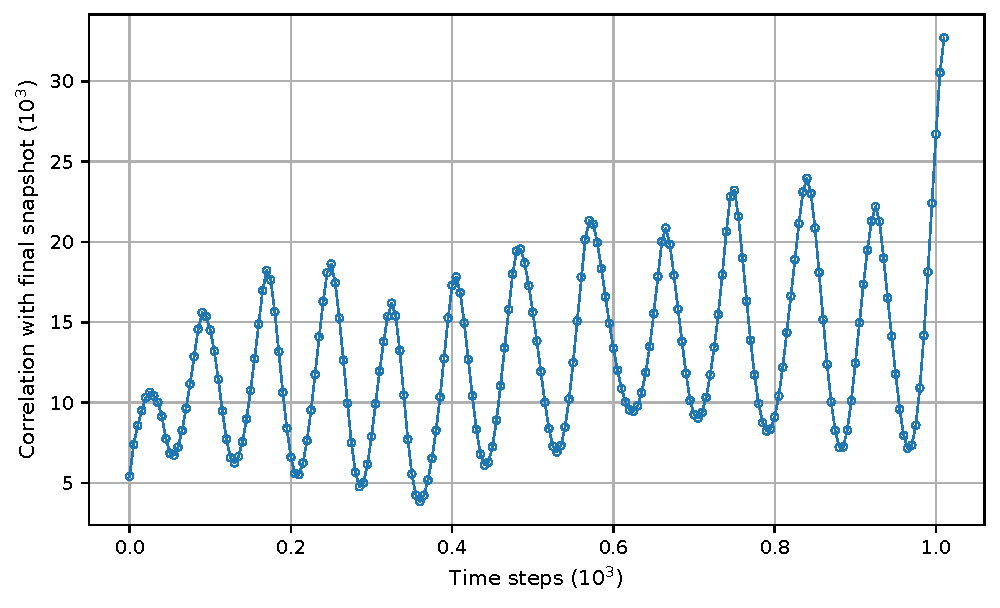
\includegraphics[width=0.7\linewidth]{figures/figure2_autocorrelation.pdf}}
\caption{Correlation between each frame and the last one, in the worst-case scenario (highest speed with a Reynolds number of $10^4$ and smallest distance $h/D$ of $0.44$).}
\label{fig1}
\end{figure}

Since a periodic segment could not be selected consistently, POD was applied to the full snapshot sequence for all simulations. The same full-sequence procedure was also applied to the canonical reference case to keep the comparison methodologically consistent.

\subsection{Sensitivity to Reynolds Number}
\label{subsec4.2}
For Reynolds numbers $Re \geq 2000$, reconstruction error exhibited only weak dependence on Reynolds number, as shown in \hyperref[fig2]{figure~3}. This finding indicates that spontaneous changes in swimming speed, such as acceleration or deceleration, would not, in isolation, cause POD-based reconstruction errors to be impossible to track over the course of an experiment. For Reynolds numbers below 2000, reconstruction error exhibited a strong dependence on Re, yet since this regime lies outside the range relevant to this study, it was not analyzed further.

\begin{figure}[]
\centering{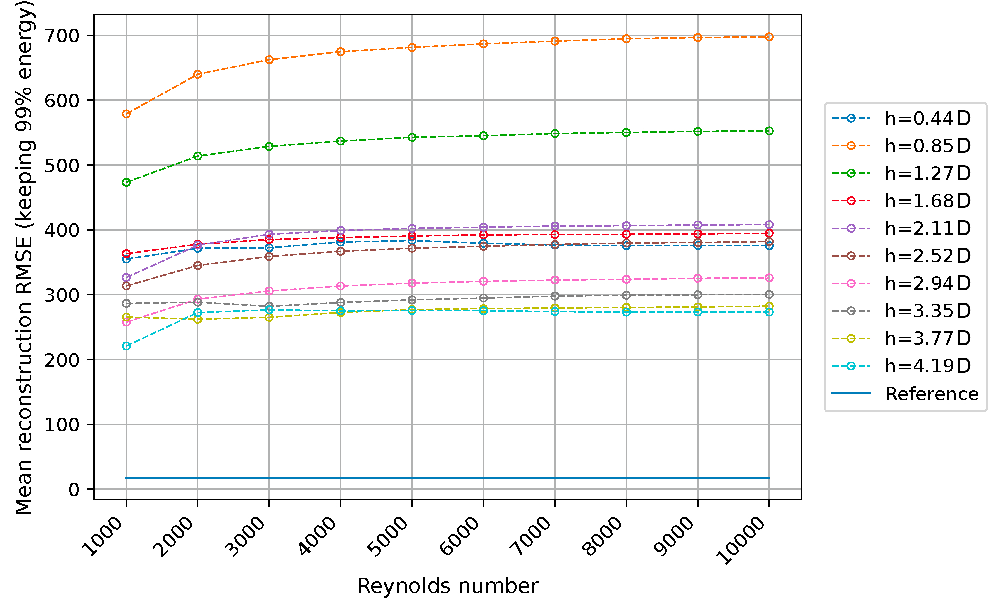
\includegraphics[width=0.7\linewidth]{figures/figure3_rmse_vs_re.pdf}}
\caption{Evolution of the mean RMSE of reconstruction with 99\% of the initial kinetic energy with respect to the Reynolds number for the 10 available distances $h$. The reference corresponds to the unbounded, stationary cylinder wake at Re = $10^2$ analyzed by Noack et al.~\citep{Noack2003}, in periodic regime.}
\label{fig2}
\end{figure}

This result provided an encouraging indication of the robustness of POD in dynamically evolving conditions typical of fish locomotion.

Additionally, the same figure revealed a more pronounced sensitivity of reconstruction error to wall proximity. This observation motivated the subsequent analysis, which is aimed at characterizing the nature of this dependency in detail.

\subsection{Strong Nonlinear Dependence on Wall Proximity}
\label{subsec4.3}
Wall proximity emerged as a dominant factor influencing POD reconstruction performance. Reconstruction RMSE increased by up to a factor of two in response to relatively small changes in the gap between the cylinder and the wall.

Three distinct flow regimes were identified (\hyperref[fig3]{figure~4}), consistent with the wall-gap mechanisms reported in the literature but not intended as exact replications of those threshold values. The relevant physical picture is that the wall first suppresses or strongly distorts the gap-side shear layer, then allows intermittent or asymmetric shedding as the gap opens, and finally approaches a weakly confined wake at larger gaps \citep{Price2002}:
\begin{itemize}
    \item Small gap regime ($h/D \leq 0.44$): strong wall interaction, inhibited gap-side circulation and loss of regular alternate shedding.
    \item Intermediate gap regime ($0.44 < h/D \leq 1.68$): circulation exists on both sides of the cylinder, but the wake remains asymmetric and sensitive to wall-induced secondary structures.
    \item Large gap regime ($h/D > 1.68$): the wake approaches the unbounded-cylinder organization, although residual wall effects remain in the finite tank.
\end{itemize}

\begin{figure}[]
\centering{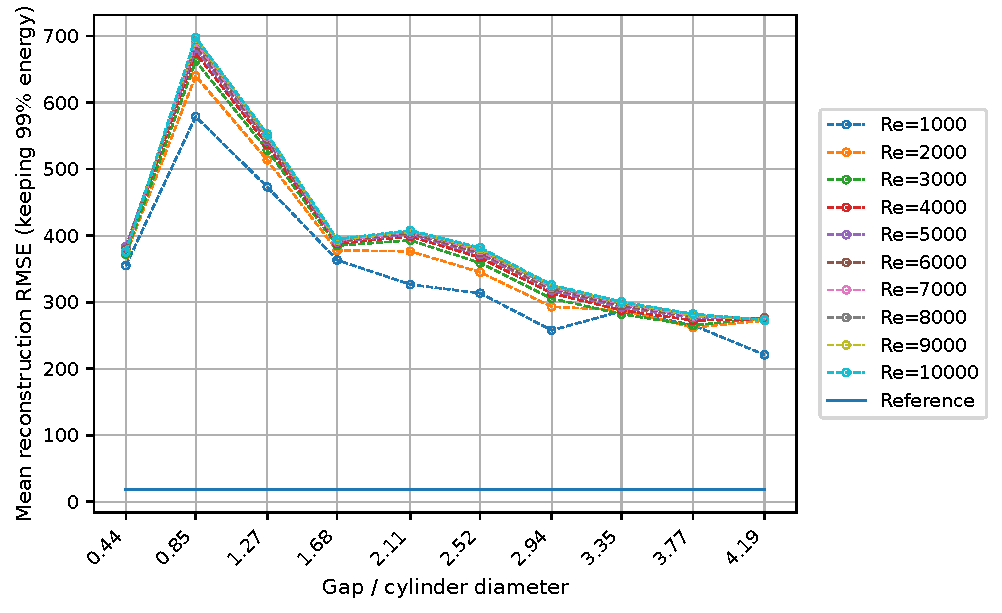
\includegraphics[width=0.7\linewidth]{figures/figure1_rmse_vs_gap.pdf}}
\caption{Evolution of the mean RMSE of reconstruction with 99\% of the initial kinetic energy with respect to the distance between the cylinder and the wall divided by the diameter of the cylinder for the 10 available Reynolds number $Re$ and the reference scenario.}
\label{fig3}
\end{figure}

Although the number of proximity values sampled in certain regimes, particularly the small-gap regime, was limited, the trend was sufficiently pronounced to confirm a strong and nonlinear sensitivity of POD reconstruction to wall proximity.

This sensitivity is not inherently problematic in controlled scenarios where position is known precisely or motion is constrained to near-linear trajectories. However, in the broader context of hydrodynamic sensing in freely swimming fish, it poses a significant challenge. This is due to two compounding factors: (i) fish frequently operate within the small- and intermediate-gap regimes, and (ii) wall proximity cannot be measured with sufficient precision to prevent high uncertainty in reconstruction quality. As a result, small errors in estimating the fish's distance to the wall can lead to unpredictable and potentially chaotic variations in reconstruction accuracy, thereby compromising data fusion reliability.

\subsection{Windowing and Resolution Effects}
\label{subsec4.4}
Spatial windowing was found to consistently degrade POD reconstruction accuracy, as illustrated in \hyperref[fig4]{figure~5}. This effect was observed regardless of whether windowing was applied a priori (before POD computation) or a posteriori (after global decomposition). These findings indicated that spatial cropping is not a viable strategy for mitigating the increase in reconstruction error induced by wall proximity.

\begin{figure}[]
\centering{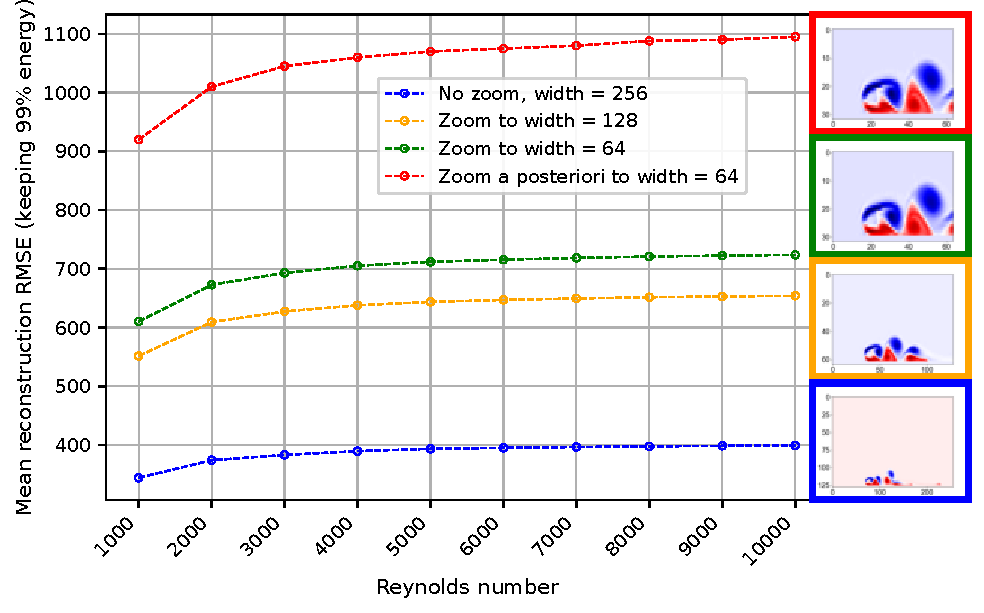
\includegraphics[width=0.7\linewidth]{figures/zoom.pdf}}
\caption {Evolution of the mean RMSE of reconstruction with 99\% of the initial kinetic energy with respect to the Reynolds number averaged over the 10 available distances, for four windowing scenarios.}
\label{fig4}
\end{figure}

Furthermore, windowing did not enable a viable sliding-window rebase strategy to emulate non-moving scenarios in the presence of body motion. As such, it fails to compensate for reconstruction errors which could potentially be arising from translational dynamics or wall-induced distortion.

Doubling the spatial resolution of the simulation led to modest improvements in reconstruction accuracy, reducing RMSE by less than a factor of two (\hyperref[fig5]{figure~6}). However, this improvement came at the cost of approximately four times the computational load. As a result, the trade-off between computational efficiency and reconstruction fidelity did not favor the use of higher resolution in this context.

\begin{figure}[]
\centering{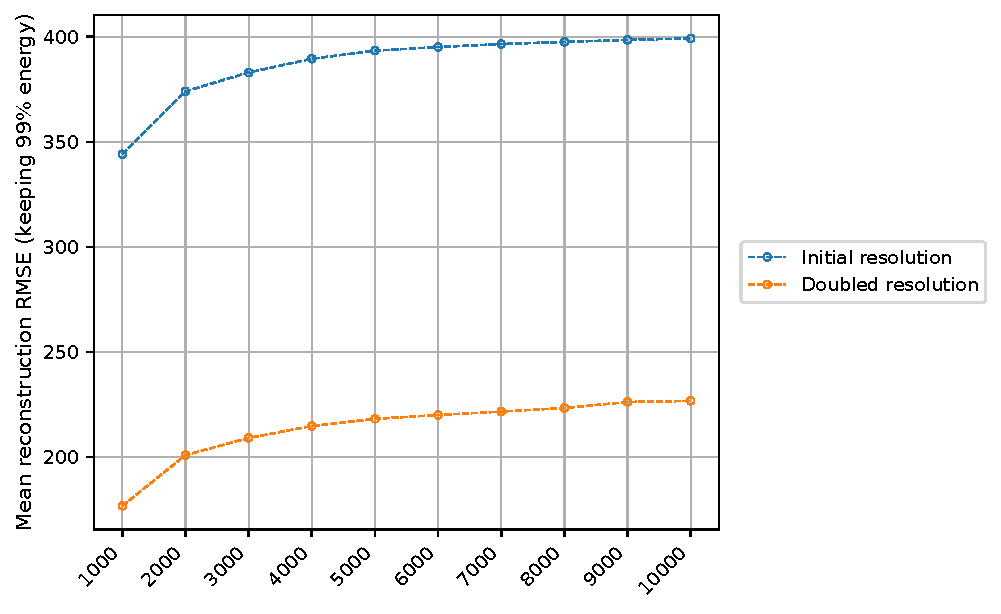
\includegraphics[width=0.7\linewidth]{figures/resolution.pdf}}
\caption {Evolution of the mean RMSE of reconstruction with 99\% of the initial kinetic energy with respect to the distance between the cylinder and the wall divided by the diameter of the cylinder averaged on the 10 available Reynolds numbers for two resolutions.}
\label{fig5}
\end{figure}

\subsection{Translating Cylinder}
\label{subsec4.5}
When simulation durations were matched by cropping the default cases to the same time span, translating-cylinder scenarios produced reconstruction errors approximately 33\% higher than their fixed-cylinder counterparts (\hyperref[fig6]{figure~7}). This confirmed that body translation introduces additional complexity that impairs POD reconstruction accuracy.

\begin{figure}[]
\centering
\begin{overpic}[width=0.95\linewidth]{figures/translation_side_by_side.pdf}
  \put(27,35.5){\makebox(0,0){\textbf{Moving cylinder}}}
  \put(74,35.5){\makebox(0,0){\textbf{Static cylinder}}}
\end{overpic}
\caption {Evolution of the mean RMSE of reconstruction with 99$\%$ of the initial kinetic energy with respect to the distance between the cylinder and the wall divided by the diameter of the cylinder for the 10 available Reynolds numbers $Re$ and the reference scenario for a moving cylinder in initially still water (left side) against default setup with a similarly cropped duration (right side).}
\label{fig6}
\end{figure}

However, the increase in error appeared primarily as an offset rather than a change in trend. The overall dependency of reconstruction error on wall proximity remained consistent between translating and stationary configurations. This suggested that, although POD reconstruction degrades under body motion, it does not exhibit a strong sensitivity to translational effects per se.

This comparison between fixed and translating cases also highlighted the specific impact of transients. While the motion itself exerted limited influence, scenarios focusing on the early, non-periodic phase of the flow (despite the absence of a clear pseudo-steady regime) showed a substantial reduction in reconstruction error. In fact, reconstruction RMSE values in these transient segments were an order of magnitude lower than those in the full-duration stationary cases. For wall distances beyond 2.94 cylinder diameters, reconstruction errors were even lower than those reported in the canonical unbounded scenario analyzed by Noack, suggesting that much of the error in classical setups originates from reconstructions over the "steady-state" regime.

The focus on transient phases also revealed different flow regime characteristics relative to wall proximity. In these cases, the small-gap and intermediate regimes appeared to blend more smoothly. Moreover, a regime shift was observed: in translating scenarios, the threshold between intermediate and large-gap regimes shifted toward larger distances, occurring at approximately $1.27$ cylinder diameters.

\subsection{Sparse wall-pressure reconstruction}
\label{subsec4.6}
The benchmark tested whether the pressure field could be recovered from the eight wall-pressure samples that motivate the data-fusion workflow, and whether regime-local bases described in Table~\ref{tab:sparse_dataset} improved either oracle full-field projection or sparse gappy reconstruction. The comparison is shown against wall gap in Figure~\ref{fig:sparse_gap} and against Reynolds number in Figure~\ref{fig:sparse_re}. Table~\ref{tab:sparse_methods} summarizes the full test set.

\begin{table}[]
\centering
\caption{Gap-regime grouping identified from the POD sensitivity analysis and used for the regime-local sparse-pressure reconstructions.}
\label{tab:sparse_dataset}
\begin{tabular}{lcc}
\toprule
Regime & Cases & Gap range \\
\midrule
Small gap & 10 & 0.44 \\
Intermediate gap & 30 & 0.85--1.68 \\
Large gap & 60 & 2.11--4.19 \\
\bottomrule
\end{tabular}
\end{table}

\begin{figure}[]
\centering{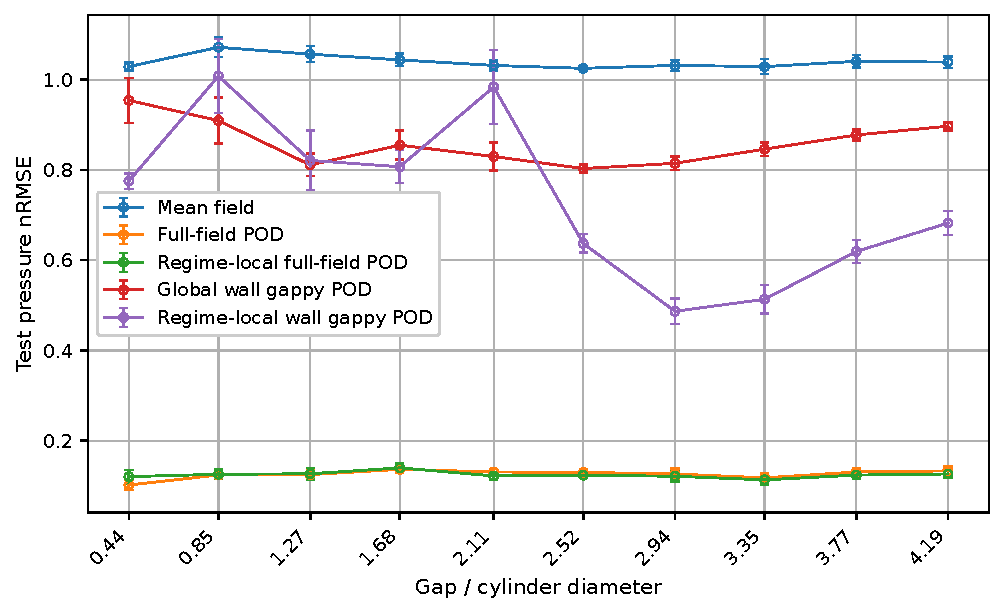
\includegraphics[width=0.78\linewidth]{figures/sparse_pressure_methods_vs_gap.pdf}}
\caption{Pressure reconstruction error as a function of normalized wall gap, averaged over Reynolds number. Full-field POD curves are oracle projections. Gappy POD curves use eight wall sensors. Error bars denote the standard deviation over the ten Reynolds-number cases.}
\label{fig:sparse_gap}
\end{figure}

\begin{figure}[]
\centering{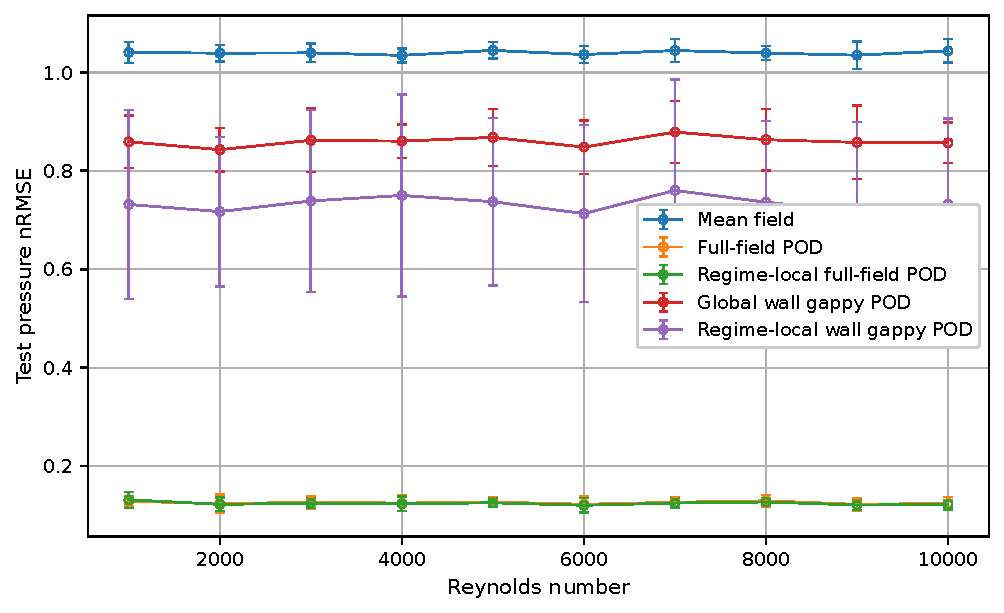
\includegraphics[width=0.78\linewidth]{figures/sparse_pressure_methods_vs_re.pdf}}
\caption{Pressure reconstruction error as a function of Reynolds number, averaged over wall gap. Full-field POD curves are oracle projections. Gappy POD curves use eight wall sensors. Error bars denote the standard deviation over the ten wall-gap cases.}
\label{fig:sparse_re}
\end{figure}

\begin{table}[]
\centering
\caption{Pressure reconstruction summary over the 100 stationary pressure-map cases. Full-field POD methods are oracle projections. Wall gappy POD methods use the eight wall sensors. The nRMSE is computed on held-out test snapshots.}
\label{tab:sparse_methods}
\begingroup
\small
\setlength{\tabcolsep}{4pt}
\resizebox{\linewidth}{!}{%
\begin{tabular}{lcccc}
\toprule
Method & Mean nRMSE & Max nRMSE & Sensor residual nRMSE & Median $\kappa(H\Phi_r)$ \\
\midrule
Mean field & 1.040 & 1.110 & -- & -- \\
Full-field POD & 0.125 & 0.146 & -- & -- \\
Regime-local full-field POD & 0.124 & 0.155 & -- & -- \\
Global wall gappy POD & 0.860 & 0.999 & 0.516 & 41.078 \\
Regime-local wall gappy POD & 0.733 & 1.111 & 0.233 & 2.279 \\
\bottomrule
\end{tabular}
}
\endgroup
\end{table}

The 99\% training-variance criterion selected 184 modes for the global full-field pressure basis. The regime-local full-field ranks were 25, 66 and 116 modes for the small-, intermediate- and large-gap groups, respectively. Validation selected eight modes for the global gappy basis and seven, five and six modes for the small-, intermediate- and large-gap local gappy bases, respectively.

Global full-field POD projection reduced the average pressure nRMSE from 1.040 for the mean-field baseline to 0.125, confirming that the pressure maps retain low-dimensional structure when the full field is available. Regime-local full-field POD gave a comparable mean nRMSE of 0.124. By contrast, global gappy POD from eight wall sensors achieved an average nRMSE of 0.860. This was better than the mean field but remained far from the global full-field projection error. The gap-resolved curves showed that global wall gappy POD remains weakest at the smallest gap, where the average nRMSE reaches about 0.95.

The Reynolds-number curves were comparatively flat. For global wall gappy POD, the average nRMSE varied only from 0.843 to 0.879 across $Re=10^3-10^4$. This mirrored the earlier POD sensitivity observation that Reynolds number is not the dominant source of reconstruction variability in the sampled range.

The local basis improved the sparse reconstruction in the average case. Regime-local gappy POD reduced the mean nRMSE to 0.733 and lowered the sensor residual nRMSE from 0.516 to 0.233. The condition-number diagnostic in Figure~\ref{fig:sparse_condition} is consistent with this improvement: the median condition number of $H\Phi_r$ decreased from 41.1 for the global gappy basis to 2.3 for the regime-local bases. The improvement was not uniform, however, as the worst local-gappy cases reached an nRMSE of about 1.11 near both regime boundaries, at the small-to-intermediate and intermediate-to-large transitions. Adapting the basis to wall-gap regimes therefore improves the sparse inverse problem, while leaving regime-transition cases as a practical source of fragility.

\begin{figure}[]
\centering{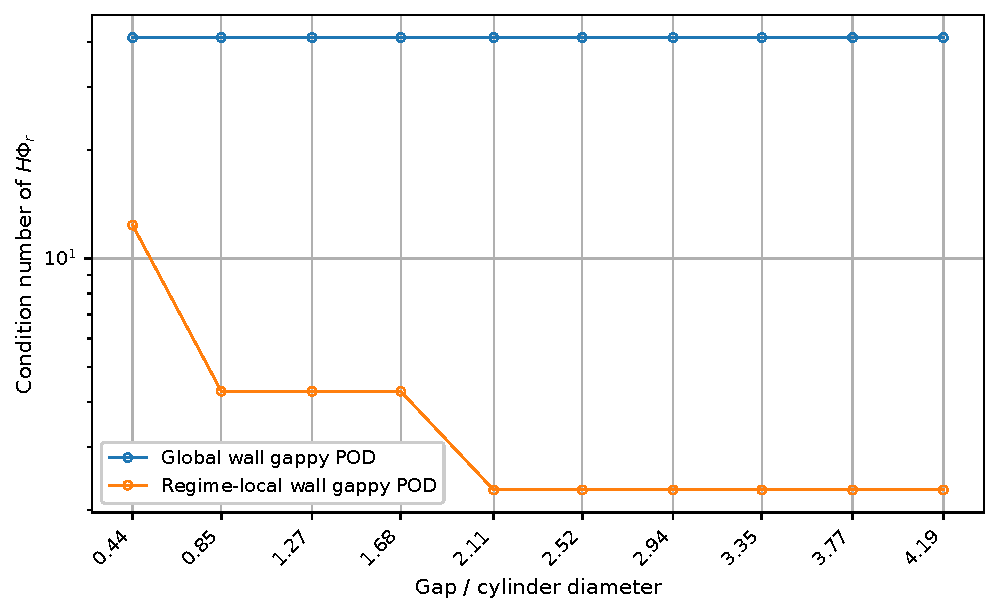
\includegraphics[width=0.78\linewidth]{figures/sparse_pressure_condition_vs_gap.pdf}}
\caption{Condition number of the sparse sensor-to-mode matrix $H\Phi_r$ as a function of wall gap. With validation-selected gappy ranks, the regime-local bases reduce the condition number relative to the global basis across all gap groups.}
\label{fig:sparse_condition}
\end{figure}

\section{Discussion}
\label{sec5}
\subsection{Implication for POD-based data fusion}
\label{subsec5.1}
Although the sensitivity of wake dynamics to wall proximity is well documented, its consequences for POD-based data fusion are less frequently addressed. In hydrodynamic sensing applications, this sensitivity poses a critical challenge: the quality of a POD-based reduced-order representation becomes strongly dependent on wall distance, a parameter that is difficult to estimate accurately in experiments.

For freely swimming fish, wall proximity can vary continuously during a trial and may only be coarsely inferred from video data. Under such conditions, small uncertainties in position translate into large and difficult-to-predict variations in reconstruction error, undermining the stability required for downstream tasks such as system identification or sensor fusion.

The breakdown of periodicity in confined, high-Reynolds-number wakes further compromises classical POD workflows. Unlike canonical cylinder wakes, most confined flows do not consistently exhibit quasi-periodic regimes, forcing POD to operate on strongly transient data and preventing its restricted application or shift mode supplementation, as in the canonical example of Noack et al.~\citep{Noack2003}. As a result, POD may not provide a sufficiently stable foundation for interpretable data fusion pipelines such as POD-SINDy in the present context.

The sparse pressure benchmark adds a second constraint. Even when a POD basis represents the pressure field better than the mean field, the associated coefficients may not be fully observable from wall pressure alone. Using 99\% training-variance ranks for full-field projection and validation-selected ranks for gappy POD, global and regime-local full-field POD produced similar oracle projection errors. Regime-local bases also improved wall-sensor gappy POD and reduced the median condition number of the sensor-to-mode map. However, the remaining gap between regime-local gappy POD and regime-local full-field POD shows that sensor placement still limits how much of the modal information can be recovered from the wall. Such a loss of information is expected when only eight wall-mounted measurements are available. Increasing the number of sensors could improve observability, but the constraint that measurements remain wall-mounted is central to the non-invasive character of the fish experiments and cannot be removed as easily as in an unconstrained sensor-placement study.

\subsection{Limitations of the present study}
\label{subsec5.2}
The present study deliberately adopts a simplified configuration in order to isolate the impact of confinement and transience on POD robustness. All simulations are two-dimensional and involve rigid cylindrical geometries, so they do not resolve three-dimensional wake instabilities or body deformation present in real fish locomotion. This remains an important limitation at $Re=10^3-10^4$, since circular-cylinder wakes are known to transition to three-dimensional dynamics at much lower Reynolds numbers \citep{Williamson1996}. However, as mentioned earlier, the two-dimensional approximation is not arbitrary in the present hydrodynamic-sensing context: low-frequency disturbances generated by swimming fish have been shown to be well represented by coherent, nearly two-dimensional vortical structures \citep{Hanke2000}, and the Cartesian-grid method underlying LilyPad has been validated up to $Re=10^5$ \citep{Maertens2015}.

In addition, the parameter space is sampled with the objective of detecting sensitivity rather than exhaustively characterizing regime boundaries. The identification of flow regimes with respect to wall proximity is therefore qualitative and intended to support interpretation rather than to provide precise classification thresholds.

Finally, the analysis focuses on POD as a front-end for data fusion and system identification, rather than on optimizing sensor placement or proposing a new assimilation algorithm. More advanced placement strategies, adaptive dictionaries or nonlinear estimators may improve reconstruction quality in specific scenarios. The present result is narrower: a straightforward energy-based POD front-end can benefit from regime-local bases, but the tested wall-sensor configuration still does not recover the accuracy available when full-field coefficients are known.


\subsection{Outlook: alternative modeling strategies}
\label{subsec5.3}
The limitations identified in this case study motivate the exploration of alternative modeling approaches capable of accommodating strong nonlinearity, regime transitions, and heterogeneous boundary effects. In particular, data-driven methods based on nonlinear latent representations offer a promising direction.

Autoencoder architectures, including variational autoencoders, provide a means of learning low-dimensional latent spaces that capture shared features across heterogeneous data sources \citep{Su2024}. Such representations may better capture the continuous deformation of flow structures induced by wall effects and body motion by enabling fusion of low-fidelity CFD-derived fields and sparse and noisy sensor data. More recently, diffusion-based generative models have demonstrated strong performance in scientific modeling. GenCast, introduced by Price et al.~\citep{Price2025}, outperforms traditional numerical models in complex meteorological tasks while preserving power spectra, which is an essential requirement for physical fidelity. The relevance of diffusion models to flow field fusion has also been supported by recent contributions such as Huang et al.~\citep{Huang2024} and Qiu et al.~\citep{Qiu2024}, all of which point to the adaptability of these architectures for combining multi-fidelity or multimodal scientific data.

It would thus be of significant interest to apply those modern techniques to the reconstruction and analysis of flow fields generated by freely swimming fish, but a major limitation lies in the volume of training data required. Addressing this requirement will likely necessitate coordinated efforts to construct larger, standardized datasets combining experimental measurements and numerical simulations across a wide range of confined flow scenarios. Such datasets would not only support the development of more expressive models, but also enable systematic evaluation of their robustness under realistic experimental constraints.

\section{Conclusions}
\label{sec6}
This case study examined the robustness of POD in wall-confined, unsteady flows representative of experimental tank conditions in biological hydrodynamics. Four main findings emerge.

First, beyond moderate values, Reynolds number does not constitute the dominant source of instability in POD-based reconstructions. For Reynolds numbers in the range $\mathcal{O}(10^3-10^4)$, reconstruction error shows only weak sensitivity to changes in flow speed, suggesting that variations in swimming speed alone are unlikely to cause severe degradation of POD-based representations in this regime.

Second, wall proximity is identified as the primary driver of reconstruction instability. POD reconstruction error exhibits a strong and nonlinear dependence on the distance to the nearest solid boundary, with small changes in proximity producing large variations in reconstruction quality. The emergence of distinct proximity-dependent regimes, consistent with established hydrodynamic classifications, indicates that this behavior reflects genuine physical transitions rather than numerical artifacts.

Third, mitigation strategies such as spatial windowing, increased spatial resolution, or accounting for body translation do not fundamentally resolve this instability. While increased resolution yields modest improvements and translation affects absolute error levels, neither approach mitigates the dominant influence of wall proximity.

Fourth, sparse wall-pressure reconstruction benefits from adapting the POD basis to wall-gap regimes. Regime-local gappy POD substantially improved reconstruction relative to a global gappy basis, suggesting that, for a freely swimming fish whose distance to the wall varies during a trial, sparse reconstruction may not require an exact continuous estimate of wall distance but could instead rely on a coarser regime label. However, the nonlinear transition between gaps remains a limitation and cases near regime boundaries may be difficult to assign reliably. As a result, gappy POD does not meet the stability needed for data fusion in the context of the broader freely swimming fish analysis.

These conclusions are specific to confined, transient, two-dimensional conditions examined in this case study. POD remains effective in canonical configurations with weak boundary effects and stationary regimes, but its underlying assumptions are poorly matched to strongly confined experimental environments. By delineating these limits of applicability, this case study highlights the need for alternative modeling approaches capable of supporting robust data fusion in heterogeneous, data-scarce and dynamically evolving flow conditions. Ultimately, advancing hydrodynamic data fusion in biologically realistic conditions will depend on modeling tools that balance physical interpretability with expressive capacity while explicitly accounting for sparse observability.

\section*{Declaration of competing interest}
The authors declare that they have no known competing financial interests or personal relationships that could have appeared to influence the work reported in this paper.

\section*{CRediT authorship contribution statement}
\textbf{Bastien Lagneaux:} Conceptualization, Methodology, Software, Validation, Formal analysis, Investigation, Writing - Original Draft, Writing - Review \& Editing, Visualization.
\textbf{Corentin Porcon:} Methodology, Ressources, Writing - Review \& Editing.
\textbf{Florence Razan:} Writing - Review \& Editing, Supervision.
\textbf{Dixia Fan:} Writing - Review \& Editing, Supervision, Project administration, Funding acquisition.
\textbf{Gurvan Jodin:} Writing - Review \& Editing, Supervision, Project administration, Funding acquisition.

\section*{Data availability}
Due to the size of the dataset, it is not possible to make it publicly available. However, the authors are willing to share the dataset upon request.

\section*{Acknowledgements}
This work was supported by a Research Grant from HFSP: \url{https://doi.org/10.52044/HFSP.RGY00592022.pc.gr.153593}.

\section*{Declaration of generative AI and AI-assisted technologies in the manuscript preparation process}
During the preparation of this work, the authors used ChatGPT-5.5 (OpenAI) in order to improve language, readability, and reduce French-influenced phrasing. After using this tool, the authors reviewed and edited the content as needed and take full responsibility for the content of the publication.

\bibliographystyle{elsarticle-num}
\bibliography{references}

\end{document}

%%\endinput
%%
%% End of file `elsarticle-template-num.tex'.
